\documentclass{article}
\usepackage[utf8]{inputenc}
\usepackage{graphicx}
\graphicspath{ {./images/} }
\usepackage{amsmath}
\usepackage{hyperref}
%\usepackage[english]{babel}

\usepackage[left=2cm,right=1cm, top=2cm,bottom=2cm,bindingoffset=0cm]{geometry}

\renewcommand{\normalsize}{\fontsize{14}{18pt}\selectfont}

\title{Studying antibiotic resistance via alignment and variants detection}
\author{  Ignat Sonets, Kamilla Faizullina}
\date{\empty}

\begin{document}


\maketitle
In this project, we analyze sequencing data from a strain of E. coli in order to find variants which could lead to the resistance to the antibiotic ampicillin. We use open-source tools to process data and detect mutations. We found the positions of variants in the genome and suggest the possible effects of each mutations. 

\section{Introduction}
Antibiotics are the powerful drugs which used to treat or prevent some types of bacterial infection. However, the enormous and irresponsible use of the antibiotics  has contributed significantly to the advent of the resistant strains \cite{anti}, \cite{anti2}. Development of new antibiotics can be helpful. To that end, scientists carry out researches related to mechanism of resistance. 
\\
In this work, we use the set of real sequencing data from a strain of E.coli resistant to the antibiotic ampicillin in order to analyze it and detect single-nucleotide polymorphism (SNP). The project aims to find the mutated genes to research the mechanism of resistance and attempt to  make recommendations for alternative antibiotics. 
 
\section{Methods}
\subsection{Data}

\begin{table}[h!]
	\centering
	\begin{tabular}{||c c ||} 
		\hline
		Sequencing data  &  Number of reads    \\ [0.5ex] 
		\hline\hline
		Original  & 455876    \\ 
		Trimmed & 446259 \\ [1ex] 
		\hline
	\end{tabular}
	\caption{Number of reads }
	\label{table:reads}
\end{table}



First, We use the reference  sequence of the  Escherichia coli strain \cite{datalink}. This is E.coli strain K-12 substrain MG1655, laboratory workhorse.  Second, we use the sequencing data of an E. coli strain which is resistant to the antibiotic ampicillin \cite{datalink_res}.

We use Fastqc for the quality control \cite{fqc} (See \ref{sec:supplement}).  With the aim to improve the overall quality of the sequencing data Trimmomatic tool is applied \cite{trim}. We cut off  off the start and the end of a read if quality below 20. We also drop the reads if their lengths are below 20. The window size is 10 and  the average quality  within the window 20. 

 Both forward and reverse initial data consist of 455876 reads. The improved data contains 446259 reads.  \\

\subsection{Aligning sequences to reference}
As we need to map the data from the resistant strain to the reference sequence, we use the aligner called BWA-MEM \cite{bwa}. In order to prepare the data we use \cite{sam}. This utility allows to index and sort bam-format files.

VarScan is used to find SNP \cite{var}. VarScan allows to change the threshold which regulates if  the position is called mutation. We decided to use --min-var-frequency=0.95. 

\section{Results}
First, we improve sequencing data quality of the resistant strain and index data. After, we align the sequence from resistant strain to the reference sequence to detect variants. 
 

The filtered data is used to detect the variants. Five variants is found. 

\begin{table}[h!]
\centering
\begin{tabular}{||c c c c c c  ||} 
 \hline
Position  & Ref & Alt  & Ref Amino acid & Alt  Amino acid & Gene   \\ [0.5ex] 
 \hline\hline
93043 & C & G & A &  G& ftsI \\ 
482698 & T & A  & Q & L  & arcB  \\
852762 & A & G & - & - & rybA \\
3535147 & A & C & V& A&  envZ \\ 
4390754 & G & T & A& T&  rsgA \\ [1ex] 
 \hline
\end{tabular}
\caption{Results }
\label{table:2}
\end{table}


\section{Discussion}
%Position 852762 does not codes protein according to NCNI \cite{ncbi}.
%
%The changing in position 852762 could affect the EG11704 (EcoCyc) which codes multidrug efflux pump RND permease AcrB. This is the inner membrane component of a tripartite.
%
%The variants in position 3535147 could change the gene  EG10269 (EcoCyc). This is the member of the two-component regulatory system EnvZ/OmpR.
%
%Mutation in position 93043 affects the gene G7841 (EcoCyc) which codes small ribosomal subunit biogenesis GTPase RsgA. RsgA induces local conformational changes in the 30S subunit and may thereby destabilize kinetically trapped assembly intermediates
%
%Mutation in position 93043 affects the gene EG10341 (EcoCyc) \cite{ecocyc}. This part of the genome decodes FtsI (penicillin-binding protein 3, PBP3) \cite{uniprot}. Penicillin-binding protein is essential cell division protein that catalyzes cross-linking of the peptidoglycan cell wall at the division septum. The variants of this gene could make strain resistant to antibiotic.

Let's discuss our findings.
We found 5 SNPs, 3 of them could probably explain antibiotic resistance. You can find additional info in Table 2 (position, changes, amino acid changes).

First thing we found is FtsI mutation.
FtsI is an essential cell division protein that catalyzes cross-linking of the peptidoglycan cell wall at the division septum. Required for localization of FtsN.
Inhibited by beta-lactam antibiotics such as penicillin, moenomycin, macarbomycin, furazlocillin and piperacillin. Antibiotics inhibit the activity by binding to the catalytic serine. Binding of beta-lactam antibiotics to FtsI inhibits FtsI activity and is lethal for the cell. So, mutation in ftsI is obligatory in evolving AMR. Interruption in ftsI-antibiotic binding will do the job. Similar results were obtained for H. influenzae \cite{bwamsnotes}.

ArcB is the sensor histidine kinase of the ArcAB two-component system which mediates anaerobic repression of numerous enzymes associated with aerobic metabolism. ArcB is an integral membrane protein with a significant cytoplasmic domain; the protein contains two transmembrane regions and three cytoplasmic modules — a primary transmitter module with a conserved histidine residue (His-292), a receiver module with a conserved aspartate residue (Asp-576) and an alternative transmitter module with a conserved histidine (His-717). Purified, soluble ArcB (lacking the two transmembrane domains) autophosphorylates in the presence of ATP and transfers a phosphate to its cognate response regulator ArcA. ArcA (accroding to scientific results) is crucial for evolving AMR \cite{amr}. Disrupting ArcA work will cause increased tetracycline susceptibility \cite{sucs}. In our case we guess that SNP in arcB gene caused no damage, but additional research to confirm our ideas required.

We also found RybA mutation.
The ~205 nt small RNA RybA was later found to encode the small protein MntS. Manganese toxicity upon overexpression was shown to be due to MntS rather than RybA.
RybA expression is upregulated under peroxide stress conditions. Apparently, the mature 207 nt rybA transcript is stabilized under peroxide stress.
RybA appears to regulate expression of genes for aromatic amino acid biosynthesis. Under peroxide stress, it acts as a negative regulator for expression of aroL and aroF by an unknown mechanism that involves TyrR. In addition, gene expression analysis suggests that RybA acts as a positive regulator for the CusR regulon. It's difficult to say that RybA somehow participates in an antibiotic resistance mechanisms. We suggest that this mutation could enhance survivability under stress conditions, but does nothing for antibiotic resistance itself.

EnvZ is a member of the two-component regulatory system EnvZ/OmpR involved in osmoregulation (particularly of genes ompF and ompC) as well as other genes. EnvZ functions as a membrane-associated protein kinase that phosphorylates OmpR in response to environmental signals; at low osmolarity OmpR activates ompF transcription, while at high osmolarity it represses ompF and activates ompC transcription. The cytoplasmic dimerization domain (CDD) forms an osmosensitive core; increasing osmolarity stabilizes this segment (possibly by its contraction), enhancing the autophosphorylation rate and consequently, downstream phosphotransfer to OmpR and signaling. Autophosphorylation is inhibited by the angucycline antibiotic waldiomycin in a non-competitive manner; waldiomycin prevents dimerization of the cytoplasmic domain and autophosphorylation. There are a number of reports describing porine regulation via EnvZ/OmpR during cell envelope stress. To put in simple, we can interpret mutation effect as porin alterations and, as a result, hampering of the drug accumulation inside cells under the threshold for bacterial death. We think that the mutation in envZ as an additional one, which increases resistance, but does not provide it entirely. Also, direct mutation of EnvZ protein can alter proper antibiotics-EnvZ binding and thus cause AMR.
The last SNP we found is RsgA. It's one of at least 4 proteins (Era, RbfA, RimM and RsgA/YjeQ) that assist in the late maturation steps of the functional core of the 30S ribosomal subunit. RsgA binds the 30S subunit contacting the head, platform, and rRNA helix 44, which may assist the last maturation stages. The GTPase activity is inhibited by aminoglycoside antibiotics such as neomycin and paromycin streptomycin and spectinomycin. This inhibition is not due to competition for binding sites on the 30S or 70S ribosome. So, mutations in RsgA can affect antibiotic therapy efficiency. Accroding to this article, deletion of RsgA significantly delayed mortality \cite{pubmed}. In our case we suggest that this mutation can prevent antibiotics binding and thus negate the effects of the therapy.


According to general mechanisms of resistance, we suggest that in our case at least 2 mechanisms involved:
1) target site alteration(for ftsI);
2) reducing drug amount in cell(for envZ).
For other SNPs additional research is required.
What about treatment and managing therapy? There are not so many working options. AMR is a complex problem that requires a united multisectoral approach.
First, limiting the usage of antibiotics as much as possible. It includes preventing self-medication and clinical misuse. To prevent misuse in clinical practice, new rapid and affordable methods for antibiotic sensitivity detection should be used. It should be noted, that limitation of use of antibiotics in livestock should be use. For clinical practice architectural replanning of the hospitals and clinics should be preformed ASAP to prevent occurrence of nosocomial infection.
And finally we want to mention therapy. Instead of conventional antibiotics vaccines and/or viruses, such as phages, can be used. Microorganisms do not develop resistance to vaccines because a vaccine enhances the body's immune system, whereas an antibiotic operates separately from the body's normal defenses. Furthermore, if the use of vaccines increases, there is evidence that antibiotic resistant strains of pathogens will decrease; the need for antibiotics will naturally decrease as vaccines prevent infection before it occurs. Phages can be bioengineered to target multidrug-resistant bacterial infections, and their use involves the added benefit of preventing the elimination of beneficial bacteria in the human body.
Another option is alternating therapy. It is a method in which two or three antibiotics are taken in a rotation versus taking just one antibiotic such that bacteria resistant to one antibiotic are killed when the next antibiotic is taken. Studies have found that this method reduces the rate at which antibiotic resistant bacteria emerge in vitro relative to a single drug for the entire duration. Nevertheless we came alternate therapy not only using 2+ antibiotics, but modify treatment using additional drugs. For example, using clavulonic acid together with beta-lactam antibiotics greatly improves their efficiency because of action of clavulonic acid(inhibitor of beta-lactamase).
One more way to deal with AMR is developing new drugs. And there bioinformatics may(and can, and should!) help. The drug discovery process is time-consuming, expensive and laborious. The traditionally available drug discovery process initiates with the identification of the target as well as the most promising drug molecule, followed by the optimization of this, in vitro, in vivo and in preclinical studies to decide whether the compound has the potential to be developed as a drug molecule. Drug discovery, drug development and commercialization are complicated processes. To overcome some of these problems, there are many computational tools available for new drug discovery, which could be cost-effective and less time-consuming. In silico approaches can reduce the number of potential compounds from hundreds of thousands to the tens of thousands which could be studied for drug discovery and this results in savings of time, money and human resources.



 \section{Supplement}
 \subsection{Improvement of the overall quality of the initial data}
 \label{sec:supplement}
\begin{figure}[h]

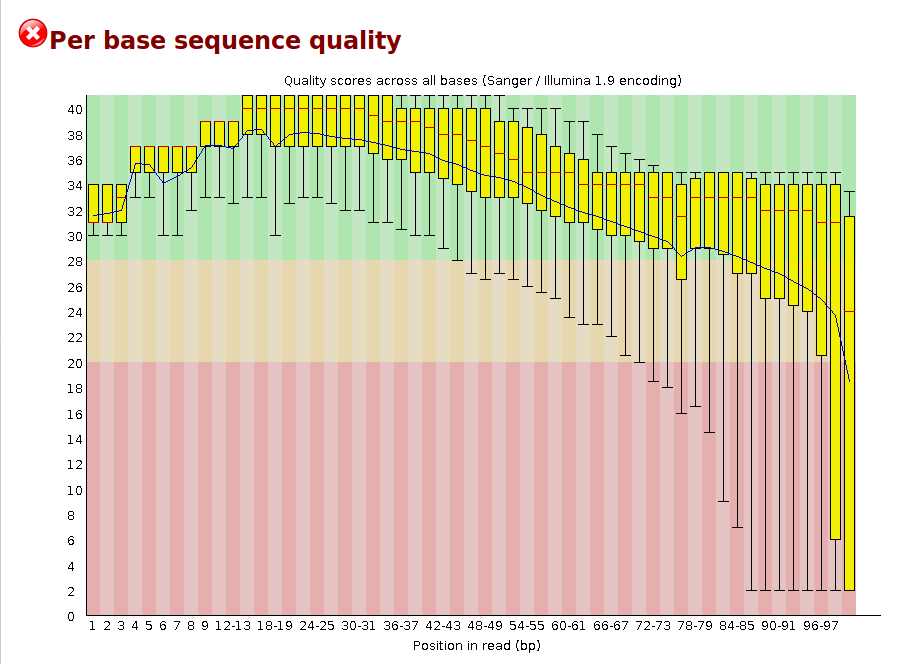
\includegraphics[scale=0.35]{fow_prev_trim.png} 
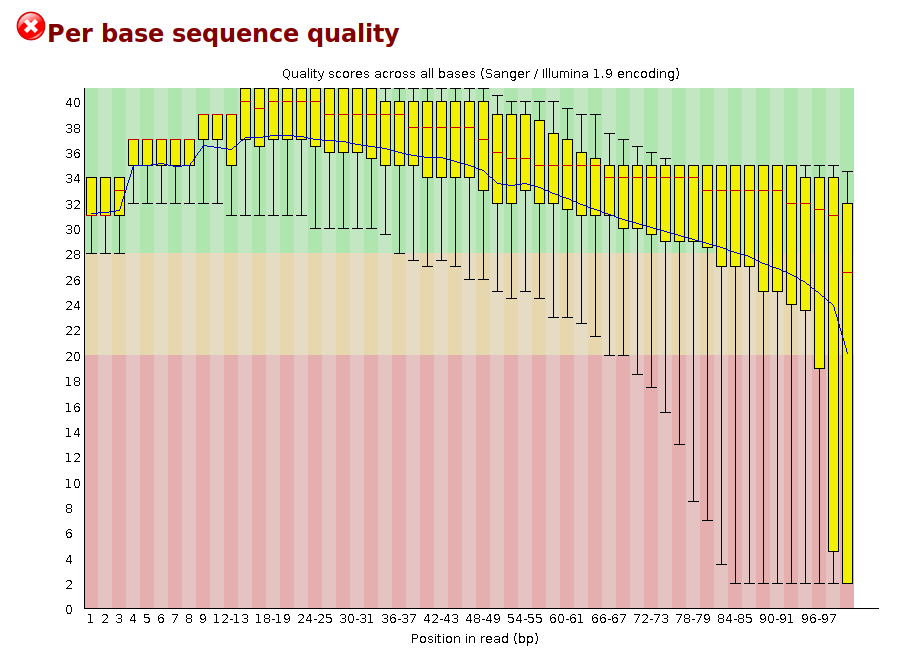
\includegraphics[scale=0.35]{rev_prev_trim.png} \\
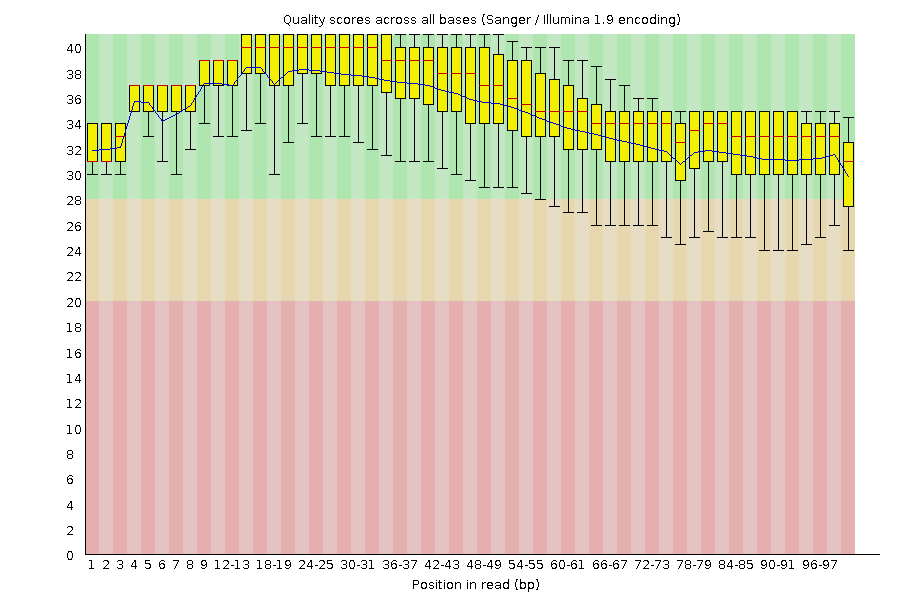
\includegraphics[scale=0.35]{fow_aft_trim.png}
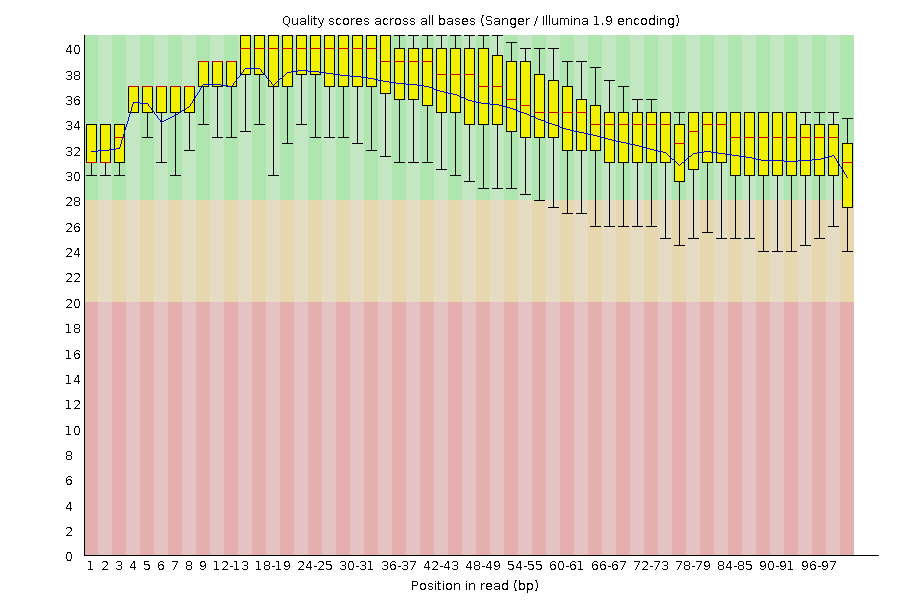
\includegraphics[scale=0.35]{rev_aft_trim.png}
\caption{ The quality of forward (left) and reverse (right) sequence before and after applying Trimmomatic  }
\label{saw}
\end{figure}


\newpage
\begin{thebibliography}{9}

\bibitem{anti} 
Zaman SB, Hussain MA, Nye R, Mehta V, Mamun KT, Hossain N. A Review on Antibiotic Resistance: Alarm Bells are Ringing. Cureus. 2017;9(6):e1403. Published 2017 Jun 28. doi:10.7759/cureus.1403 

\bibitem{anti2}
Ventola CL. The antibiotic resistance crisis: part 1: causes and threats. P T. 2015;40(4):277–283. 

\bibitem{datalink}
The reference data, retrieved  from \href{ftp://ftp.ncbi.nlm.nih.gov/genomes/all/GCA/000/005/845/GCA_000005845.2_ASM584v2}{NCBI FTP}
 
 
\bibitem{datalink_res}
The data of resistant strains:  \href{http://public.dobzhanskycenter.ru/mrayko/amp_res_1.fastq.zip}{first} and 
\href{http://public.dobzhanskycenter.ru/mrayko/amp_res_2.fastq.zip}{second} 

\bibitem{fqc}
%\href{https://www.bioinformatics.babraham.ac.uk/projects/fastqc/}{Fastqc}
Andrews, S. (2010). FastQC:  A Quality Control Tool for High Throughput Sequence Data [Online]. Available online at: http://www.bioinformatics.babraham.ac.uk/projects/fastqc/

\bibitem{trim}
%\href{http://www.usadellab.org/cms/?page=trimmomatic}{Trimmomatic: A flexible read trimming tool for Illumina NGS data}
Bolger, A. M., Lohse, M., Usadel, B. (2014). Trimmomatic: A flexible trimmer for Illumina Sequence Data. Bioinformatics, btu170.

\bibitem{bwa}
%\href{http://bio-bwa.sourceforge.net/}{Burrows-Wheeler Aligner}
Li H. and Durbin R. (2010) Fast and accurate long-read alignment with Burrows-Wheeler Transform. Bioinformatics, Epub. [PMID: 20080505] 

\bibitem{sam}
%\href{http://samtools.sourceforge.net/}{SAM (Sequence Alignment Map) }
Heng Li, Bob Handsaker, Alec Wysoker, Tim Fennell, Jue Ruan, Nils Homer, Gabor Marth, Goncalo Abecasis, Richard Durbin, 1000 Genome Project Data Processing Subgroup, The Sequence Alignment/Map format and SAMtools, Bioinformatics, Volume 25, Issue 16, 15 August 2009, Pages 2078–2079, https://doi.org/10.1093/bioinformatics/btp352

\bibitem{var}
%\href{http://dkoboldt.github.io/varscan/}{VarScan }
Koboldt, D., Zhang, Q., Larson, D., Shen, D., McLellan, M., Lin, L., Miller, C., Mardis, E., Ding, L., Wilson, R. (2012). VarScan 2: Somatic mutation and copy number alteration discovery in cancer by exome sequencing Genome Research DOI: 10.1101/gr.129684.111
URL: http://varscan.sourceforge.net 

 \bibitem{ncbi}
%\href{ https://www.ncbi.nlm.nih.gov/nuccore/NC_000913.3?report=graph}{NCBI }
 National Center for Biotechnology Information (NCBI)[Internet]. Bethesda (MD): National Library of Medicine (US), National Center for Biotechnology Information; [1988] – [cited 2017 Apr 06]. Available from: https://www.ncbi.nlm.nih.gov/
 
 \bibitem{ecocyc}
%\href{https://biocyc.org/gene?orgid=ECOLI&id=EG10341}{EcoCyc }
Ingrid M. Keseler, Amanda Mackie, Alberto Santos-Zavaleta, Richard Billington, César Bonavides-Martínez, Ron Caspi, Carol Fulcher, Socorro Gama-Castro, Anamika Kothari, Markus Krummenacker, Mario Latendresse, Luis Muñiz-Rascado, Quang Ong, Suzanne Paley, Martin Peralta-Gil, Pallavi Subhraveti, David A. Velázquez-Ramírez, Daniel Weaver, Julio Collado-Vides, Ian Paulsen, Peter D. Karp, The EcoCyc database: reflecting new knowledge about Escherichia coli K-12, Nucleic Acids Research, Volume 45, Issue D1, January 2017, Pages D543–D550, https://doi.org/10.1093/nar/gkw1003

 \bibitem{uniprot}
%\href{https://www.uniprot.org/uniprot/P0AD68}{UniProt}
The UniProt Consortium, UniProt: a worldwide hub of protein knowledge, Nucleic Acids Research, Volume 47, Issue D1, 08 January 2019, Pages D506–D515, https://doi.org/10.1093/nar/gky1049

 \bibitem{bwamsnotes}
Misawa, K., Tarumoto, N., Tamura, S. et al. Single nucleotide polymorphisms in genes encoding penicillin-binding proteins in beta-lactamase-negative ampicillin-resistant Haemophilus influenzae in Japan. BMC Res Notes 11, 53 (2018). https://doi.org/10.1186/s13104-018-3169-0

\bibitem{susc}
Mario L. Arrieta-Ortiz, Min Pan, Amardeep Kaur, Vivek Srinivas, Ananya Dash, Selva Rupa Christinal Immanuel, Nitin S. Baliga.  Disrupting the ArcA regulatory network increases tetracycline susceptibility of TetR Escherichia coli. 
bioRxiv 2020.08.31.275693; doi: https://doi.org/10.1101/2020.08.31.275693 

\bibitem{amr}
Horinouchi, T., Maeda, T., Kotani, H. et al. Suppression of antibiotic resistance evolution by single-gene deletion. Sci Rep 10, 4178 (2020). https://doi.org/10.1038/s41598-020-60663-6

\bibitem{pubmed}
Rocchio S, Santorelli D, Rinaldo S, Franceschini M, Malatesta F, Imperi F, Federici L, Travaglini-Allocatelli C, Di Matteo A. Structural and functional investigation of the Small Ribosomal Subunit Biogenesis GTPase A (RsgA) from Pseudomonas aeruginosa. FEBS J. 2019 Nov;286(21):4245-4260. doi: 10.1111/febs.14959. Epub 2019 Jul 2. PMID: 31199072.

\end{thebibliography}

\end{document}
